\chapter{SPECTRE attacks}

	\begin{wrapfigure}{l}{0.4\textwidth}
		
\includegraphics[width=0.38\textwidth]{spectre}
		\caption{Il logo di SPECTRE}
		\label{fig:spectre}
	\end{wrapfigure}

	\index{Spectre}In questo capitolo verrà presentato il progetto \emph{SPECTRE}\cite{kocher2018spectre} (il cui logo è rappresentato in \cref{fig:spectre}), una famiglia di attacchi molto recenti che sfruttano una vulnerabilità presente nella maggior parte dei processori moderni (Intel, AMD e ARM) e per i quali, al momento attuale, non esistono contromisure tranne l'utilizzo di alcuni accorgimenti in fase di programmazione come vedremo più avanti.
	
	Si parla di famiglia di attacchi perché di questo attacco esistono cinque varianti, tutti documentati con il proprio codice \ac{CVE} nello \emph{Standard for Information Security Vulnerability Names} gestito dalla \href{https://www.mitre.org/}{MITRE Corporation}. Le varianti sono le seguenti:
	
	\begin{itemize}
		\item [v1:] bounds check bypass \href{https://cve.mitre.org/cgi-bin/cvename.cgi?name=CVE-2017-5753}{(CVE-2017-5753)}
		\item [v2:] branch target injection \href{https://cve.mitre.org/cgi-bin/cvename.cgi?name=CVE-2017-5715}{(CVE-2017-5715)}
		\item [v3:] using speculative reads of inaccessible data \href{https://cve.mitre.org/cgi-bin/cvename.cgi?name=CVE-2017-5754}{(CVE-2017-5754)}
		\item [v3a:] using speculative reads of inaccessible data, aka "rogue system register read" \href{https://cve.mitre.org/cgi-bin/cvename.cgi?name=CVE-2018-3640}{(CVE-2018-3640)}
		\item [v4:] speculative bypassing of stores by younger loads despite the presence of a dependency \href{https://cve.mitre.org/cgi-bin/cvename.cgi?name=CVE-2018-3639}{(CVE-2018-3639)}
	\end{itemize}
	
	Nel resto di questo lavoro ci focalizzeremo sulla prima variante di questa tipologia di attacchi.
	
	La caratteristica che viene sfruttata principalmente in questa variante è la cosiddetta \emph{esecuzione speculativa}, una funzione presente in quasi tutti i processori moderni.
	
	\section{Esecuzione speculativa}
		\index{Esecuzione speculativa}L'esecuzione speculativa è una tecnica utilizzata dai processori per ottenere un miglioramento delle prestazioni; essa consiste nel cercare di "indovinare" il risultato di un branch basandosi sui risultati ottenuti in precedenza, per poter eseguire anticipatamente alcune istruzioni.
		
		Immaginiamo di essere in campo durante la finale del mondiale di calcio. Stiamo battendo il rigore decisivo. Abbiamo studiato bene il portiere avversario nell'ultimo anno e sappiamo che le 10 volte in cui gli si è presentato davanti un tiratore mancino (come lo siamo noi) si è sempre tuffato alla sua sinistra ed ha sempre parato il rigore. Avendo fiducia nel nostro studio decidiamo di calciare alla sua destra in maniera non troppo angolata, per non rischiare di sbagliare, certi comunque di spiazzarlo. Sfortunatamente però, questa volta il portiere decide di cambiare angolo e para facilmente il nostro rigore facendoci perdere il mondiale.
		
		Quale è stata la cosa che ci ha fatto sbagliare? L'aver speculato sul comportamento del portiere ed aver pensato che il fatto che si fosse sempre tuffato a sinistra nelle occasioni precedenti ed avesse sempre parato il rigore, lo avrebbe portato a farlo di nuovo. Vediamo come riportare questo esempio nel nostro ambito. 
		
		Supponiamo ad esempio che l'esecuzione di un programma dipenda da un controllo su di un valore non presente in cache che quindi deve essere recuperato dalla memoria principale. Questo può portare ad un attesa di svariate centinaia di cicli di clock. Invece di aspettare tutto questo tempo inutilmente, il processore cerca di indovinare il risultato del controllo, salva lo stato attuale dei suoi registri, e procede ad eseguire speculativamente il ramo del branch che ritiene più plausibile (supponiamo il ramo then). Quando poi arriverà il valore effettivo dalla memoria, verrà eseguito il controllo. Se il risultato è quello aspettato (true nel nostro caso), si prosegue con la computazione e saranno stati risparmiati tutti quei cicli di clock che sarebbero stati persi nell'attesa. Se la scelta si rivela sbagliata (false), il processore scarta tutti i risultati dell'esecuzione speculativa, si riporta allo stato che aveva salvato prima del branch ed esegue l'altro ramo (else).
		
		Questa ottimizzazione sembra perfetta in quanto in caso di successo, si risparmiano molti cicli di clock mentre in caso di insuccesso il risultato è paragonabile a quello che avremmo ottenuto aspettando il dato senza eseguire alcuna istruzione. Purtroppo vedremo che non è così.
		
		Il responsabile di questa scelta è una piccola unità all'interno del processore chiamata \ac{BP}.
		
		\subsection{Branch predictor}
			\index{Branch Predictor}Esistono svariati tipi di branch predictor; analizziamo il funzionamento di uno dei più semplici, il \emph{one-level branch predictor}\index{One-level branch predictor} a 2 bit.
			
			\begin{figure}
				\begin{center}
					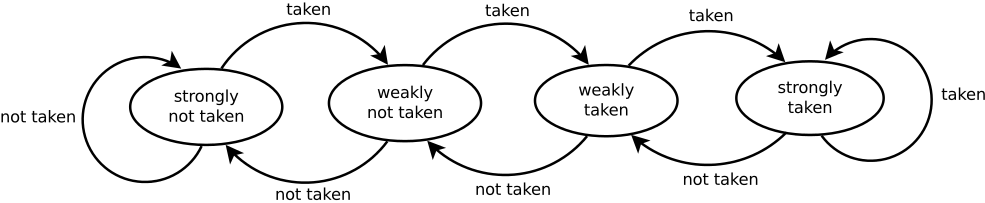
\includegraphics[scale=.35]{bp2bit}
					\caption{Automa di decisione di un one-level branch predictor a 2 bit}
					\label{fig:bp2bits}
				\end{center}
			\end{figure}
		
			Come da schema in \cref{fig:bp2bits} un one-level branch predictor può essere descritto con un semplice automa a 4 stati.
			
			\begin{enumerate}
				\item \emph{Strongly not taken:} in questo stato il \ac{BP} sceglierà il ramo else del branch. In caso di conferma negativa del controllo resterà in questo stato altrimenti passerà allo stato 2.
				\item \emph{Weakly not taken:} in questo stato il \ac{BP} ha già osservato una esecuzione then ma la sua scelta resterà ancora il ramo else. Se il controllo si rivelerà false, il \ac{BP} tornerà allo stato 1 ma se si rivelerà true andrà allo stato 3 dal quale inizierà a scegliere il ramo then.
				\item \emph{Weakly taken:} come detto in precedenza, in questo stato il \ac{BP} inizierà a scegliere il ramo then. Se da questo stato si ottiene un false, torneremo allo stato 2, altrimenti passeremo al 4.
				\item \emph{Strongly taken:} questo stato è il duale dello stato 1. In questa situazione il \ac{BP} sceglierà il ramo then rimanendo in questo stato se otterrà un true e tornando allo stato 3 se otterrà un false (continuando comunque ad eseguire il ramo then).
			\end{enumerate}
		
			In questo caso vediamo come l'esecuzione consecutiva di al più due rami then ci porta sicuramente in uno stato in cui la prossima scelta del \ac{BP} sarà sicuramente il ramo then. Questa informazione sarà molto utile quando dovremo effettuare un training sul \ac{BP} per convincerlo a prendere una certa decisione quando si troverà davanti ad un certo branch.
			
	\section{L'attacco}
		L'attacco SPECTRE induce la vittima ad eseguire speculativamente operazioni che non dovrebbero essere eseguite durante l'esecuzione corretta del programma. Da tali operazioni si otterranno poi le informazioni ricercate tramite un side-channel temporale.
		
		L'attacco si può scomporre in tre fasi:
		
		\begin{enumerate}
			\item \emph{Fase di setup:} in questa fase l'attaccante esegue delle operazioni che convincono il \ac{BP} ad eseguire il ramo then in caso si rendesse necessaria una esecuzione speculativa. In questa fase si cerca anche di costruire tale necessità ad esempio eseguendo letture di memoria che rimuovono dalla cache un valore che sarà poi necessario successivamente. Come ultima cosa l'attaccante può iniziare a preparare la porzione di cache dalla quale estrarrà il valore che vuole carpire alla vittima (ad esempio eseguendo il flush o l'evict di una line o di un set).
			\item \emph{Esecuzione speculativa:} in questa fase il processore esegue speculativamente delle istruzioni che esporrano informazioni confidenziali della vittima recuperabili tramite un side-channel temporale. Tale esecuzione può esporre una vasta gamma di dati sensibili ma nell'articolo gli autori si concentrano sulla possibilità di recuperare un valore che risiede ad un indirizzo preciso nella memoria della vittima attraverso un attacco di tipo Flush+Reload o Evict+Reload.
			\item \emph{Recupero del dato:} come ultimo passo, viene montato l'attacco alla cache (Flush+Reload o Evict+Reload). Il recupero del dato si ottiene andando a misurare il tempo necessario alla lettura dall'indirizzo di memoria presente nella line sotto attacco.
		\end{enumerate}
	
		Vediamo adesso un esempio pratico.
		
		\subsection{Esempio}
		
			Consideriamo il caso di una funzione che riceve un intero x da una fonte non fidata (come ad esempio il \cref{list:vulnerabile}).
			
			\begin{lstlisting}[caption={Funzione sotto attacco},label={list:vulnerabile}]
				if (x < array1_size) {
					y = array2[array1[x] * 256];
				}
			\end{lstlisting}
			
			Il processo che la esegue ha accesso ad un array di bytes \emph{array1} di dimensione \emph{array1\_size} ed un secondo array, \emph{array2}, di dimensione pari a 64KB.
			
			La funzione inizia con un controllo su x, necessario per essere sicuri di non permettere la lettura di porzioni di memoria al di fuori di array1. Durante l'esecuzione speculativa di questo codice però, il \ac{BP} può selezionare il ramo then relativo a questo controllo ad esempio nel seguente caso:
			
			\begin{itemize}
				\item il valore di x viene scelto in maniera malevola in maniera tale da far puntare array1[x] ad un byte segreto \emph{k} che risiede da qualche parte nella memoria della vittima al di fuori di \emph{array1}(\cref{fig:array}).
				\item \emph{array1\_size} e \emph{array2} non sono presenti nella cache ma \emph{k} lo è.
				\item operazioni precedenti hanno restituito un valore di x corretto, addestrando il \ac{BP} a scegliere il ramo then.
			\end{itemize}
		
			Questa situazione può presentarsi in maniera normale o può essere creata dall'attaccante ad esempio leggendo grandi quantità di memoria per riempire la cache di valori completamente scorrelati ed effettuando una chiamata legittima ad una funzione che utilizzi \emph{k}.
			
			A questo punto, quando il programma inizia a girare il processore esegue il confronto tra x e \emph{array1\_size}. La lettura di \emph{array1\_size} si traduce in un cache miss ed il processore richiede il dato dalla memoria principale. Durante l'attesa il \ac{BP} assume che il risultato dell' \emph{if} sarà \emph{true}, eseguirà speculativamente la somma di x all'indirizzo base di \emph{array1} e richiederà il dato presente all'indirizzo appena calcolato. Questa operazione si tradurrà in una cache hit e verrà restituito molto velocemente il valore del byte segreto \emph{k}. L'esecuzione speculativa continua il suo percorso e verrà calcolato l'indirizzo di \emph{array2[k*256]}. La richiesta del dato contenuto a questo indirizzo si tradurrà in una cache miss e verrà richiesta una lettura dalla memoria principale. Durante questa seconda attesa, al processore arriva finalmente il valore di \emph{array1\_size}. Dopo aver eseguito il confronto il processore si accorge che l'esecuzione speculativa era errata ed esegue un rollback allo stato precedente al branch. Il problema sorge in questo momento. La richiesta di lettura rimasta sospesa viene comunque portata a termine e il valore relativo non viene rimosso dalla cache.
			
			\begin{figure}
				\begin{center}
					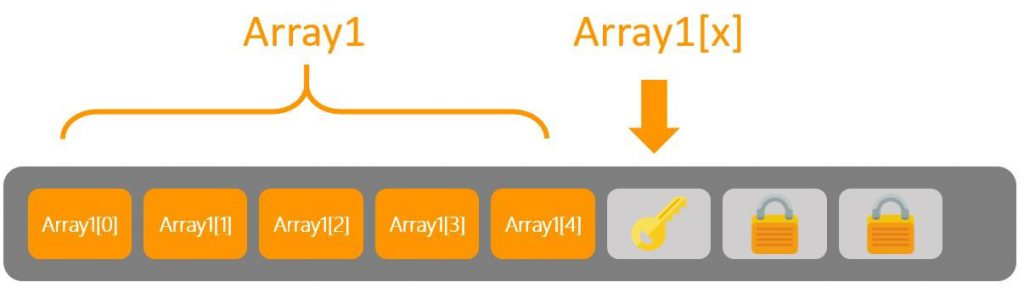
\includegraphics[scale=.3]{arraySpectre}
					\caption{Recupero del valore al di fuori di \emph{array1}}
					\label{fig:array}
				\end{center}
			\end{figure}
			
			Per completare l'attacco l'attaccante non deve fare altro che rilevare questo cambiamento nello stato della cache per recuperare il byte segreto \emph{k}.
			
			Nel caso più semplice, quello cioè in cui l'attaccante ha accesso diretto ad \emph{array2}, egli non dovrà fare altro che provare  a leggere tutte le posizioni di \emph{array2[n*256]} per tutti i valori di $n \in (0\dots255)$. Solamente uno di questi sarà presente in cache (quello per \emph{n} = \emph{k}) e verrà restituito velocemente mentre tutti gli altri verranno restituiti in tempi molto lunghi. Prendendo l'unico valore restituito in tempo breve, l'attaccante avrà trovato il byte segreto \emph{k}.
			
			Questo attacco può ovviamente essere eseguito un numero indeterminato di volte e può portare alla completa lettura della memoria della vittima un byte alla volta.
			
	\section{Le contromisure}
		Come detto all'inizio del capitolo, al momento attuale non sono state rilasciate patch a livello di hardware o di microprogrammazione del processore in grado di risolvere completamente il problema.
		
		La soluzione più ovvia è quella di non permettere l'esecuzione speculativa tout court ma questa scelta andrebbe ad impattare eccessivamente sulle prestazioni. L'idea è quella di cercare di impedire l'esecuzione speculativa su parti di codice compromettenti.
		
		In questa direzione, sia Intel che AMD, nei loro white papers \cite{AMD2018speculation,intel2018speculative}, suggeriscono alcune regole di programmazione per difendersi da questi attacchi.
		
		\subsection*{Serializzare gli accessi alla memoria}
		
		La prima regola è quella di serializzare gli accessi alla memoria tramite l'utilizzo dell'istruzione \emph{lfence()}\index{Lfence()}. Questa è un tipo di istruzione di \emph{barriera} che forza il processore o il compilatore ad una esecuzione ordinata delle operazioni di memoria richieste immediatamente prima ed immediatamente dopo la barriera. Tipicamente questo fa sì che sia garantito che l'istruzione che segue la barriera non venga eseguita prima di quella che la precede. A titolo di esempio, analizziamo il \cref{list:difendere}.
		
		\begin{lstlisting}[caption={Codice da difendere},label={list:difendere}]
			if (user_value >= LIMIT) {
				return ERROR;
			} 
			x = table[user_value]; 
			node = entry[x];
		\end{lstlisting}
		
		In questo caso, la riga 4 può essere eseguita speculativamente con il valore \emph{user\_value} fornito dall'attaccante mentre si attende il risultato del controllo presente alla riga 1, ritardato perché il valore di \emph{LIMIT} non è presente in cache. 
		
		L'istruzione \emph{lfence()} alla riga 4 del \cref{list:lfence} scongiura questa eventualità impedendo l'accesso alla memoria prima che sia terminato l'accesso precedente.
		
		\begin{lstlisting}[caption={Utilizzo di lfence},label={list:lfence}]
		if (user_value >= LIMIT) {
			return ERROR;
		} 
		lfence(); 
		x = table[user_value]; 
		node = entry[x];
		\end{lstlisting} 
		
		Questa soluzione sicuramente risolve il problema ma ha due grossi difetti; deve essere inserita manualmente a livello di programmazione e porta una perdita di prestazioni notevole\cite{AMD2018speculation}.
		
		Microsoft implementa nel proprio compilatore una rilevazione automatica del codice vulnerabile agli attacchi di tipo SPECTRE ed inserisce tali barriere automaticamente. Purtroppo la blacklist di questo strumento comprende solamente le situazioni più comuni e maggiormente utilizzate. Kocher infatti dimostra che tale analisi automatica non rileva molte sezioni di codice vulnerabile\cite{kocher2018mitigation}.
		
		\subsection*{Utilizzare variabili "volatile"}
		
		Un'altra possibile contromisura può essere quella di utilizzare variabili dichiarate \emph{volatile} come nel \cref{cod:volatile}:
		
		\begin{lstlisting}[caption={Utilizzo di variabili dichiarate volatile},label={cod:volatile}]
		volatile int user_value;
		/*
		* some untrusted operations 
		* to get the value of user_value
		*/
		if (user_value >= LIMIT) {
		return ERROR;
		} 
		x = table[user_value]; 
		node = entry[x];
		\end{lstlisting}
		
		L'attributo \emph{volatile} vieta al processore di cercare in cache il valore di variabili così dichiarate ma lo costringe a recuperarlo sempre dalla memoria principale ed evita che il compilatore esegua qualunque tipo di ottimizzazione di istruzioni contenenti tali variabili.
				
		Ovviamente anche questo metodo risolve il problema ma, come il precedente, influisce negativamente sulle prestazioni in quanto ogni volta che la variabile \emph{user\_value} viene utilizzata (anche in altri punti del programma) si dovrà sempre aspettare il suo recupero dalla memoria principale.
		
		\subsection*{Forzare le variabili entro i limiti}
		
		Questa ultima soluzione prevede di accertarsi che il valore di \emph{user\_value}, quando viene usato come indice, non vada mai a superare la dimensione del nostro array. Per ottenere questa certezza si può utilizzare l'operatore di modulo come nel \cref{list:limiti}:
		
		\begin{lstlisting}[caption={Rispetto dei limiti forzato},label={list:limiti}]
		if (user_value >= LIMIT) {
		return ERROR;
		}
		x = table[user_value % LIMIT]; 
		node = entry[x];
		\end{lstlisting}
		
		In questo caso le situazioni possibili sono due:
		
		\begin{enumerate}
			\item \emph{user\_value} è minore di \emph{LIMIT} e quindi \emph{user\_value \% LIMIT} non cambia valore.
			\item \emph{user\_value} non è minore di \emph{LIMIT} ma \emph{user\_value \% LIMIT} lo riporta entro i limiti e non può essere utilizzato per leggere memoria esterna all'array.
		\end{enumerate}
	
		Come le precedenti, anche questa soluzione funziona ma comporta un calo delle prestazioni dovuto al fatto che se la variabile \emph{LIMIT} non è in cache al momento del controllo, non lo sarà neanche quando verrà eseguita speculativamente l'istruzione della riga 4 che quindi dovrà comunque aspettare il valore corretto. 